\documentclass[11pt]{article}

\usepackage{graphicx,amsmath,amssymb,subfigure,url,xspace,float,physics}
\newcommand{\eg}{e.g.,\xspace}
\newcommand{\bigeg}{E.g.,\xspace}
\newcommand{\etal}{\textit{et~al.\xspace}}
\newcommand{\etc}{etc.\@\xspace}
\newcommand{\ie}{i.e.,\xspace}
\newcommand{\bigie}{I.e.,\xspace}

\title{Spherical Coordinates}
\author{Prajeesh A G}

\begin{document}
\maketitle

\section{Introduction}
\label{sec:into}

\begin{figure}[H]
  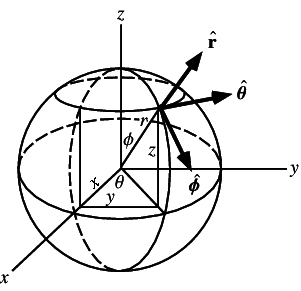
\includegraphics{SphericalCoordinates.png}

\end{figure}

Sperical Coordinates, also called Spherical polar Coordinates are a system of curvilinear Coordinates. Define $\theta$ to be the azimuthal angle in the x-y plane from the x-axis with $0 \leq \theta 2\pi$ (longitude $\lambda$ for us), $\phi$ to the polar angle (also known as zenith angle adn colatitude, with $\phi=90\deg - \delta$ where $\delta$ is the latitude in degrees) from the point to the origin. \par

\section{In terms of Cartesian coordinates}
\label{sec:cart}
The Spherical Coordinates $(r,\theta,\phi)$ are related to the cartesian Coordinates (x,y,z) by:

\begin{align}
  r &= \sqrt{x^2+y^2+z^2} \\                                                             \theta &= tan^{-1} \left(\frac{y}{x}\right) \\
  \phi &= cos^{-1} \left(\frac{z}{r}\right)
\end{align}
where $r\in(0,\infty), \theta\in(0,2\pi), \phi\in(0,\pi)$ and the inverse tangent must be suitably defined to take the correct quadrant of (x,y) into account.

In terms of Cartesian Coordinates,

\begin{align}
  \label{eq:sp2carOAt}
  x &= r\cos{\theta}\sin{\phi} \\
  y &= r\sin{\theta}\sin{\phi} \\
  z &= r\cos{\phi}
\end{align}

A line element is,

\begin{align}
  \vec{ds} &= \hat{r}dr + \hat{\phi} rd\phi + \hat{\theta} r\sin{\phi}d\theta
\end{align}

The radius vector is,

\begin{align}
  \vec{r} &= r\cos{\theta}\sin{\phi}\hat{i} + r\sin{\theta}\sin{\phi}\hat{j} + r\cos{\phi}\hat{k}
\end{align}

The unit vectors are,

\begin{align}
  \hat{r} &= \frac{\frac{d\vec{r}}{dr}}{\abs{\frac{d\vec{r}}{dr}}} \\
  \hat{\phi} &= \frac{\frac{d\vec{r}}{d\phi}}{\abs{\frac{d\vec{r}}{d\phi}}} \\
  \hat{\theta} &= \frac{\frac{d\vec{r}}{d\theta}}{\abs{\frac{d\vec{r}}{d\theta}}}
\end{align}

\bibliographystyle{plain}
\bibliography{literature.bib}

\end{document}

%%% Local Variables:
%%% mode: latex
%%% TeX-master: t
%%% End:
